Die Kurvendiskussion ist die Analyse einer Funktion im Hinblick auf ihre Eigenschaften, wie ihren \textcolor{red}{Definitionsbereich}, \textcolor{red}{Grenzwerte}, \textcolor{red}{Asymptoten}, \textcolor{red}{Schnittpunkte mit den Koordinatenachsen}, \textcolor{red}{Symmetrie}, \textcolor{red}{Extrem- und Terrassenpunkte}, \textcolor{red}{Monotonie} und ihrem \textcolor{red}{Kr"ummungsverhalten}. Die Reihenfolge spielt durchaus eine Rolle. Es macht z.B. keinen Sinn den Wertebereich vor dem Definitionsbereich zu bestimmen, da der Wertebereich direkt vom Definitionsbereich abh"angt.

\subsection{Definitons- und Wertebereich}
Wir m"ochten meist den maximalen Definitionsbereich bestimmen, den Bereich also m"oglichst wenig einschr"anken. So ist $f(x) = \frac{1}{x}$ f"ur die Zahl Null nicht definiert. Damit w"are ein m"oglicher Definitionsbereich 
\begin{equation*}
\mathbb{D} := \mathbb{R}/\{0\} = \left\{x \in \mathbb{R} \ | \ x \neq 0 \right\}
\end{equation*}
Ein ebenfalls g"ultiger Definitionsbereich w"are $\left[10;15\right]$. Solche Einschr"ankungen machen Sinn, wenn uns nur dieser Bereich der Funktion interessiert.\\
Um den Wertebereich einer Funktion $F$ zu bestimmen, bestimmen wir
\begin{equation*}
\mathbb{W}_f = f(\mathbb{D}_f) = \left\{f(x) \ | \ x \in \mathbb{D}_f \right\},
\end{equation*}
hierzu kann es vonn"oten sein zuerst die Grenzwerte (Abschnitt \ref{sec:grenzwerte}) zu betrachten.

\subsection{Schnittpunkte mit den Koordinatenachsen}
Interessant k"onnen auch die Schnittpunkte des Graphen mit den Koordinatenachsen sein, v.a. wenn man den Graphen skizzieren m"ochte.
\begin{itemize}
\item Schnittpunkt mit der y-Achse: $f(0)$, einfach einsetzten und ausrechnen.
\item Nullstellen: $f(x) = 0$ (siehe Abschnitt \ref{sec:nullstellen}).\\
Merke: Ein Polynom hat h"ochstens so viele Nullstellen wie der h"ochste Exponent der Funktion, dabei erh"alt man zum Teil auch mehrfache Nullstellen, wie beispielsweise bei $x^3$. Diese Funktion hat ein dreifache Nullstelle an der Stelle $x=0$.
\end{itemize}

\subsection{Grenzwerte} \label{sec:grenzwerte}

\begin{warning}
	Achtung: Es hei"st nicht x geht unendlich nahe an $x_0$, sondern beliebig nahe.\\
	Die Bezeichnung \textit{unendlich Nahe} existiert nicht und manche Professoren achten sehr darauf.
\end{warning}

\subsubsection{Polstellen und L"ocher}
Eine Polstelle oder ein Pol, ist eine einpunktige Definitionsl"ucke einer Funktion, wenn die Funktionswerte in jeder Umgebung des Punktes (betragsm"a"sig) beliebig gro"s werden. Der Punkt $x_0 = 1$ der Funktion $f_1$ erf"ullt dies nicht (hier handelt es sich um ein \textbf{Loch}), denn $f_1(x) = 1$ in der Umgebung von $x_0$. Betrachten wir 
\begin{equation*}
f(x) := \frac{1}{x-1}
\end{equation*}
so handelt es sich bei $x_0 = 1$ um einen Pol der Funktion $f$ da
\begin{equation*}
\lim\limits_{x \to 1^+} f(x) = \infty \text{ und } \lim\limits_{x \to 1^-} f(x) = -\infty
\end{equation*}
$1^+$ ist der \textbf{rechter Grenzwert} bei $x=1$ (ann"aherung von rechts) und $1^-$ ist der \textbf{linke Grenzwert} bei $x=1$ (ann"aherung von links). Genau dieses Verhalten, also die Grenzwerte interessieren uns bei den Polstellen.

\subsubsection{Verhalten im Unendlichen}
Nun betrachtet man das Verhalten des Graphen im Unendlichen, also
\begin{equation*}
\lim\limits_{x \to +\infty} f(x) \text{ und } \lim\limits_{x \to -\infty} f(x) .
\end{equation*}
 Dabei ist interessant, ob sich der Graph einem bestimmten Wert ann"ahert oder ob er ins Unendliche steigt oder f"allt.

\begin{warning}
	Achtet darauf das \textit{Unendlich} kein Wert ist, der einfach eingesetzt werden darf. \textit{Unendlich} kann niemals erreicht werden, dadurch kann x diesen Wert auch nicht annehmen. Man kann lediglich x gegen Unendlich gehen lassen.
\end{warning}

\subsection{Asymptoten}
Sei $f$ eine Funktion, so ist eine Asymptote von $f$ eine Gerade die $f$ im Unendlichen, in $x$ oder in $y$ Richtung, ann"ahert. Asymptoten gehen somit direkt mit den Grenzwerten der Funktion $f$ einher. Die Gerade muss keine Funktionsgerade sein! Betrachten wir erneut 
\begin{equation*}
f(x) = \frac{1}{x-1}
\end{equation*}
so ist die Gerade $x=1$ eine Asymptote von $f$. $y=0$ ist ebenfalls eine Asymptote.
%Asymptoten k"onnen Geraden aber auch andere Funktionen sein, an die sich der Graph der zu untersuchenden Funktion beliebig nah ann"ahert, ohne sie jemals zu ber"uhren. Asymptoten findet man vor allem bei gebrochen rationalen Funktionen. Dort, wo der Nenner den Wert 0 erreichen w"urde (an dieser Stelle ist die Funktion nicht definiert $=>$ Grenzwertbildung), befindet sich eine senkrechte Asymptote. Diese Stelle nennt man Polstelle. Es kann aber auch sein, dass es sich dort um ein Loch handelt, dies ist dann der Fall, wenn die Polstelle gleichsam eine Nullstelle der Funktion ist. Beispiel: $\frac{2x}{4x-1}$ Der Nenner wird 0 bei x=0.25, es handelt sich dabei um keine Nullstelle, somit befindet sich an der Stelle x=0,25 eine senkrechte Asymptote. Um den Graphen auf waagrechte oder andere Asymptoten zu untersuchen, schaut man sich die Exponenten der Variablen an. Die folgenden Ausf"uhrungen beziehen sich rein auf die h"ochsten Exponenten der Variablen im Z"ahler und Nenner.

 \subsection{Symmetrie}
 Hier untersuchen wir die Symmetrie die Graphen zum Koordinatensystem. Wir unterscheiden dabei \textbf{Punktsymmetrie} zum Koordinatenursprung und \textbf{Achsensymmetrie zur $y$-Achse}:
 \begin{itemize}
 \item Achsensymmetrie ($y$-Achse), wenn $f(x)=f(-x)$
 \item Punktsymmetrie (Ursprung), wenn $f(-x)=-f(x)$
 \end{itemize}
 siehe Abschnitt \ref{sec:symmetrie}

\subsection{Extrem- und Terrassenpunkte}
Angenommen Sie sind mit dem Auto unterwegs und sei $v(t)$ die Geschwindigkeit zum Zeitpunkt $t$. Sie beschleunigen zuerst und reduzieren anschlie"send die Beschleunigung auf $0$. Sagen wir zum Zeitpunkt $t_0$ ist die Beschleunigung gleich Null. Nun gibt es 2 M"oglichkeiten:
\begin{enumerate}
\item Sie bremsen: lokaler- oder globaler Extrempunkt von $v(t)$
\item Sie beschleunigen wieder: Terrassenpunkt bin $v(t)$
\end{enumerate}
Wenn sie bremsen (negative Beschleunigung), ist klar, dass sie zum Zeitpunkt $t_0$ eine lokale oder globale Maximalgeschwindigkeit erreicht haben. Beschleunigen sie wieder, war die Beschleunigung gleich Null, steigt dann aber wieder an. Um nun herauszufinden wann sie die maximale Geschwindigkeit erreicht haben, m"ussen wir den Zeitpunkt finden, an dem Sie beginnen zu bremsen. D.h. an dem die Beschleunigung gleich Null und somit die Ableitung von $v(t)$ gleich Null ist. Das gibt uns \textbf{m"ogliche} Punkte, es k"onnte aber sein, dass Sie wieder beschleunigt haben. Falls dies der Fall ist h"atte sich die Beschleunigung in der Umgebung um $t_0$ nicht ge"andert und damit w"are die Ableitung der Beschleunigung also die 2. Ableitung von $v$ an $t_0$ gleich Null. Andernfalls handelt es sich um den ersten Fall, also um einen Extrempunkt. Im Allgemeinen wissen wir:
\begin{equation*}
f'(x_0) = 0 \Rightarrow x_0 \text{ ist ein Extrem- oder Terrassenpunkte}
\end{equation*}
Mit der 2. Ableitung ergibt sich folgendes:
\begin{itemize}
\item $f''(x_0) = 0 \Rightarrow x_0 \text{ ist Terrassenpunkte}$ 
\item $f''(x_0) < 0 \Rightarrow x_0 \text{ ist lokales Maximum }$
\item $f''(x_0) > 0 \Rightarrow x_0 \text{ ist lokales Minimum}$
\end{itemize}
Kurz: ein lokales Maximum oder Minimum besteht immer dann, wenn die erste Ableitung an ihrer Nullstelle einen Vorzeichenwechsel hat. Andernfalls handelt es sich um einen Terrassenpunkt, dies k"onnen wir auch "uberpr"ufen ohne die 2. Ableitung zu berechnen. Achtung: Ist der Definitionsbereich eingeschr"ankt so kann ein Maximum/Minimum auch an den Definitionsgrenzen liegen. Wenn Sie von immer beschleunigen aber $v(t)$ nur bis 10 Sekunden betrachten, dann ist nat"urlich $v(10)$ ihr Maximum, aber die Ableitung ist an dieser Stelle nicht Null.
\begin{figure}[h!]
\begin{center}
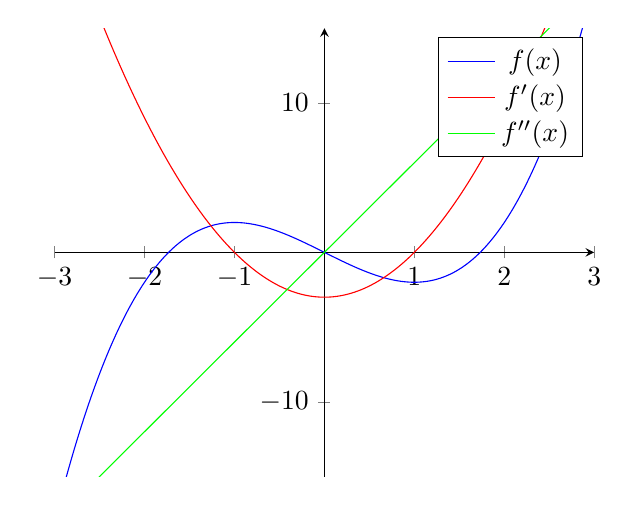
\begin{tikzpicture}[scale = 1.0]
    \begin{axis}[
        domain=-5:5,
        xmin=-3.0, xmax=3.0,
        ymin=-15, ymax=15,
        samples=400,
        axis y line=center,
        axis x line=middle,
    ]
    	   \addplot+[mark=none, color=blue] {x*x*x - 3*x};
    	   \addlegendentry{$f(x)$}
    	   \addplot+[mark=none, color=red] {3*(x*x - 1)};
    	    \addlegendentry{$f'(x)$}
    	   \addplot+[mark=none, color=green] {6*x};
    	   \addlegendentry{$f''(x)$}
    \end{axis}
\end{tikzpicture}
\end{center}
\caption{$f(x) = x^3 - 3x$, bei $x=1$ befindet sich ein lokales Minimum und bei $x=-1$ befindet sich ein lokales Maximum. Lokal da $f(3)$ ist gr"o"ser als das lokale Maximum und $f(-3)$ kleiner als das lokale Minimum. $f$ besitzt einen Wendepunkt bei $x=0$.}
\label{fig:kurvendiss}
\end{figure}

 \subsection{Monotonie}
Nachdem wir die Funktion hinreichend auf Extrem- und Terrassenpunkte untersucht haben, kann man ihre Monotonie analysieren. Diese gibt man "ublicherweise in Intervallen an, deren Grenzen die Ränder und die Extremstellen bilden. Um beim obigen Beispiel zu bleiben gibt uns die Monotonie die separierten Bereiche an denen wir Beschleunigt bzw. Abgebremst haben.

\subsection{Kr"ummung}
Um das Kr"ummungsverhalten einer Funktion zu untersuchen, ben"otigt man die zweite Ableitung des Funktionsterms. Es gilt: 
 \begin{itemize}
 \item $f''(x_0)<0 \Rightarrow f \text{ ist an } x_0 \ \textcolor{red}{rechtsgekr"ummt} $
 \item $f''(x_0)>0 \Rightarrow f \text{ ist an } x_0 \ \textcolor{red}{linksgekr"ummt}$
 \end{itemize}
Die Stelle $x_0$, an welcher der Graph seine Kr"ummung "andert, bezeichnet man als Wendepunkt, hier "andert sich die Richtung der Kr"ummung von rechts nach links, bzw. von links nach rechts. Der Wendepunkt ist gleich der Nullstelle der 2. Ableitung des Funktionsterms, d.h. die zweite Ableitung gleich $0$ setzten und den zugeh"origen $x$-Wert berechnen. Das sind die wesentlichen Schritte einer Kurvendiskussion.

 \subsection{"Ubungen}
 \begin{enumerate}
 \item Diskutiere die Kurven folgender Funktionen
 \begin{itemize}
 \item $f(x)=x^4$
 \item $f(x)=\sin(x)$
 \item $f(x)=3x^2 + 12x - 4$
 \item $f(x)=\frac{4x^3 + x^2 - x}{x+1}$
 \item $f(x)=\frac{\tan^2(x)}{\sin^2(x)}$
 \end{itemize}
 \item Untersuche folgende Funktionen auf ihre Nullstellen, Extrempunkte und Kr"ummung.
 \begin{itemize}
 \item $f(x)=(x-4)^2-3$
 \item $f(x)=(x-2)(x+5)(x-4)$
 \item $f(x)=\frac{1}{x}$
 \end{itemize}
 \end{enumerate}
 
 